\subsection{Server Recovery}
\label{sub:eval:server-recovery}

We define server recovery as the amount of time it takes for \APIName to publish a new server after a server failure.
In order to compute recovery time, we measured events related to disconnecting devices and server publication, as shown
in Listing~\ref{lst:events:server-recovery}. 


Figure~\ref{fig:server-recovery} illustrates the cumulative empirical function for server recovery time.
In most cases, server recovery is achieved within 15 seconds but there are edge cases where server recovery took almost 1 minute. 
It is worth noting that this recovery time takes into account the DNS-SD service discovery time, i.e. the time it takes for the service discovery protocol to detect that the last running service with a given name is not available anymore until a new server is published with the same name. 



\begin{figure}
    \centering
    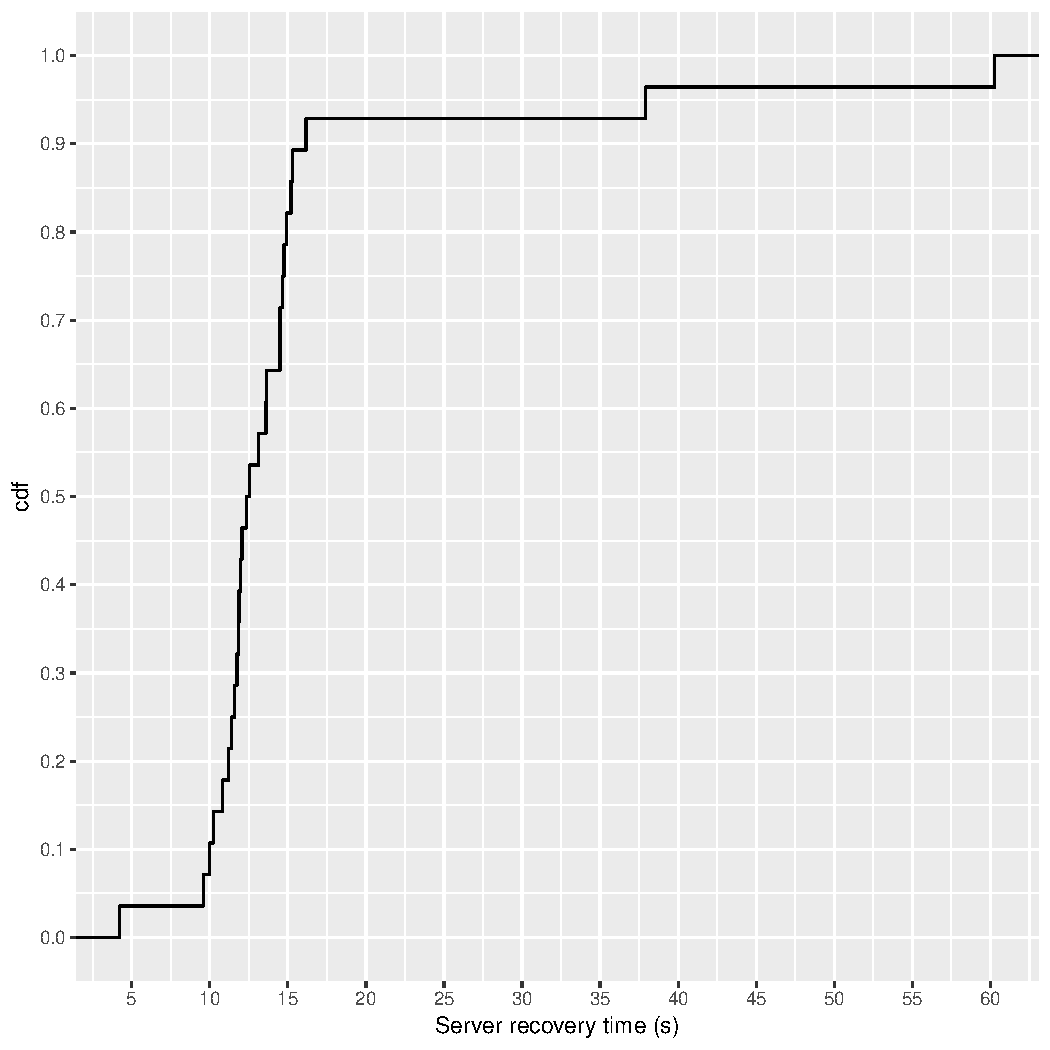
\includegraphics[width=0.9\linewidth]{server-recovery}
    \caption{Server recovery time}
    \label{fig:server-recovery}
\end{figure}


Despite recovering within 15 seconds in most cases, we acknowledge that our current recovery time should be improved for a productive version of \APINameNoSpace. 
One problematic aspect of a slow recovery is that operations cannot be applied on the shared state when clients are disconnected. 
While there are options to mitigate this problem (e.g. a client-side local queue for operations and batched submission upon re-connecting), we acknowledge that faster recovery is necessary for truly fault-tolerant local Web apps.
The performance of server recovery is mainly dictated by the implementation of service discovery in FlyWeb and we aim to research how this can be improved in the future.
For example, we could use more a aggressive protocol for service discovery~\cite{hong2007accelerating}, or, the first successor could immediately start a background ``failover server''.  
We elaborate more on potential improvements in Section~\ref{sec:limitations_and_future_work}.